\documentclass[main.tex]{subfiles}
\begin{document}

\section*{Mon Nov 04 2019}

% No lectures tomorrow, instead on Wednesday at 14.30.

\subsection{Isothermal winds with an external force}

Last time we found that the only physical solution to the stellar wind is the transsonic solution.

Now, let us add an external force:

%
\begin{align}
  v \dv{v}{r} = - \frac{1}{\rho } \dv{P}{r} - \frac{GM}{r^2} + f(r)
\,,
\end{align}
%
so we get 
%
\begin{align}
  \frac{1}{v} \dv{v}{r} = \frac{2 \frac{a^2}{r} - \frac{GM}{r^2} + f(r)}{v^2 - a^2}
\,,
\end{align}
%
with the speed of sound \(a = \sqrt{\mathcal{R} T / \mu } \). How does the velocity gradient change?
With an outward force, we expect the velocity gradient to be less steep in the subsonic region (the velocity decreases slower: the numerator is \emph{less negative}).
Adding this force is formally equivalent to modifying the gravitational field by making it weaker. This increases the pressure scale height, so the density gradient becomes less steep, so the velocity gradient becomes less steep as well.

In the supersonic region, instead the gradient will be larger: the numerator is \emph{more positive} and higher velocities are reached.

The critical radius changes: it is the solution to 
%
\begin{align}
  r_C = \frac{GM}{2 a^2} - \frac{f(r_C) r_C^2}{2 a^2}
\,,
\end{align}
%
which will shift inward as \(f\) goes from 0 to positive.

Then, we can show that the velocity at the corona must be larger: the critical radius is further inward, and the gradient is less steep.

How do we expect the mass loss rate to change? from the continuity equation at the bottom of the corona, we get \(\dot{M} = 4 \pi r_0^2 \rho_0 v_0 \), and everything on the RHS is fixed but \(v_0 \), so when we increase it the LHS must incrase as well.

Let us consider some explicit law scaling as \(f \propto r^{-2}\), like a radiative force: 
%
\begin{align}
  g _{\text{rad}} = \kappa_F \times \text{stuff} \times \qty(\frac{r}{R})^{-2}
\,.
\end{align}

This is the same as changing the mass of the star, since it scales like the gravitational force. We take our force to be \(f(r) = A / r^2\). Our equation becomes 
%
\begin{align}
  \frac{1}{v} \dv{v}{r}  = \qty(\frac{2 a^2}{r} - \frac{GM}{r^2} + \frac{A}{r^2}) / \qty(v^2- a^2)
\,,
\end{align}
%
so the effective mass is \(M _{\text{eff}} = M ( 1- A / GM)\).

This is usually called the Eddington ratio: 
%
\begin{align}
  \Gamma = \frac{A}{GM} = \frac{A/r^2}{GM / r^2}
\,,
\end{align}
%
the acceleration of the force divided by the gravitational one.

\todo[inline]{Are the units of \(A\) and \(GM\) not \SI{}{m^3 s^{-2}}?}

The critical radius becomes 
%
\begin{align}
  r_C = \frac{GM}{2a^2} \qty(1 - \Gamma )
\,,
\end{align}
%
however in general \(A\) is not taken as a constant, but activates only after a certain radius.

As \(\Gamma \) increases, the critical velocity is reached faster, and the velocity at the corona is greater.
The density profile gets less and less steep: the density scale height decreases.

\begin{figure}[H]
\centering
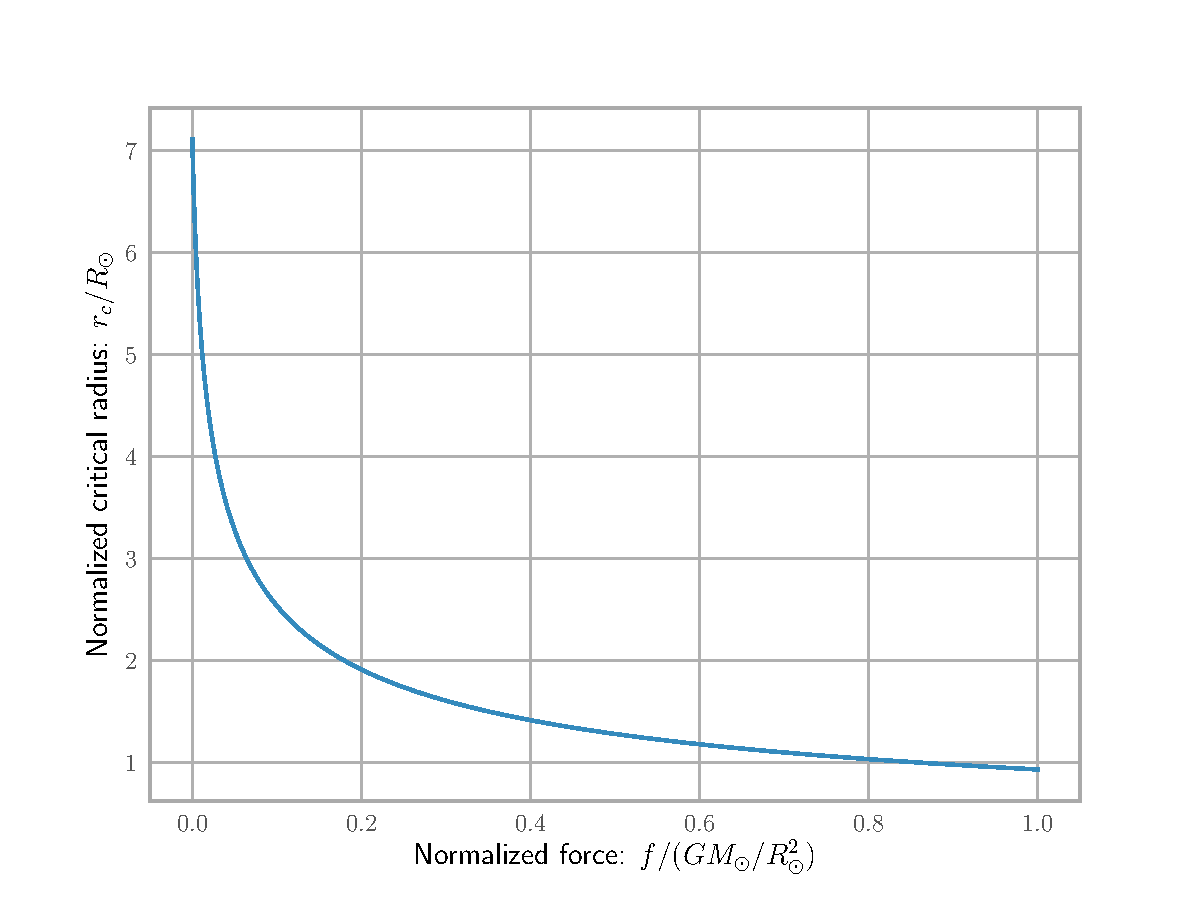
\includegraphics[width=\textwidth]{figures/critical_radius_position.pdf}
\caption{Critical radius position in function of a constant force, expressed in units of the gravitational acceleration at the surface. Here, we assume solar parameters and \(T = \SI{e6}{K}\).}
\label{fig:critical_radius_position}
\end{figure}


We approximate \(A(r) = A [r \geq r_d]\) for some \(r_d\).\footnote{Using the Iverson bracket here!}
Below the dust condensation region there is only gas, above it there is dust which is more opaque to radiation.

The critical point depends on \(\Gamma \): 
%
\begin{align}
  \frac{r_C}{1 - \Gamma (r_C)} = \frac{GM}{2 a^2}
\,.
\end{align}
%

If the extra force switches on \emph{outside} the critical region, the mass loss rate is \emph{unchanged}, since it only depends on the subsonic region.

\todo[inline]{Is there the possibility to have more than one critical radius with only outward force?}

\end{document}